\documentclass{article}
\usepackage[utf8]{inputenc}
\usepackage[brazil]{babel}
\usepackage{epsfig}
\usepackage{fancyhdr}
\usepackage{indentfirst} %In­dent first para­graph af­ter sec­tion header
\usepackage{titlesec}
\usepackage{amsmath}
\usepackage{amsthm}

\pagestyle{empty}

\headheight 40mm      %
\oddsidemargin 2.0mm  %
\evensidemargin 2.0mm %
\topmargin -40mm      %
\textheight 250mm     %
\textwidth 160mm      %
%
\newcounter{execs}
\setcounter{execs}{0}
\newcommand{\exec}[0]{\addtocounter{execs}{1}\item[\textbf{\arabic{execs}.}]}

\fancypagestyle{first}
{
\pagestyle{fancy}
}
%%%%%%%%%%%%%%%%%%%%%%%%%%%%%%%%%%%%%%%%%%%%%%%%%%%%%%%%
%%%%%%%%%%%%%%%%%%%%%%%%%%%%%%%%%%%%%%%%%%%%%%%%%%%%%%%%
% PLEASE, EDIT THIS!
\fancyhead[LO]{\small $5^a$ Lista \\ 
                DCC008 - Cálculo Numérico  \\
                \textbf{Entrega: 11 de Novembro de 2018} }

\fancyhead[RO]{\small Universidade Federal de Juiz de Fora - UFJF \\ 
                Departamento de Ciência da Computação \\
               \textit{Nome: Thiago de Almeida}\\
               \textit{Nome: Renan Nunes}}


\begin{document}
\thispagestyle{first}
%    \noindent \textbf{Obs1.:}  Escolha um ou mais métodos de interpolação dado em aula para resolver os problemas abaixo.
%    
%    \noindent \textbf{Obs2.:}  Discuta os resultados.

\begin{itemize}

\exec O arquivo ``dados.txt'' contém os dados históricos referentes a cotação diária das ações da empresa Petrobras (PETR4) nos últimos 2 anos, que são negociadas na bolsa de valores de São Paulo (BOVESPA). 

\begin{itemize}

\item[a)] Apresente gráficos comparando os dados do arquivo ``dados.txt'' com as curvas ajustadas pelo método de mínimos quadrados para diferentes ordens polinomiais ($P_n(x)$, $n=1,3,5,10,15,20,50,100$).

\item[b)] Definindo como $x$ a primeira coluna e $y$ a segunda coluna do arquivo ``dados.txt'', calcule, para todos as ordens polinomiais do item (a), o coeficiente de determinação $r$ que pode ser calculado como:
$$
r^2= 1 - \dfrac{\displaystyle \sum_{i=1}^{k} \left(y_i-P_n(x_i) \right)^2}{\displaystyle \sum_{i=1}^{k} y_i^2 - \dfrac{1}{k} \left(\sum_{i=1}^{k} y_i \right)^2 }
$$
onde $k$ denota a quantidade de dados do arquivo ``dados.txt''. Monte uma tabela apresentando os resultados do coeficiente de determinação $r$ em porcentagem ($r*100$).

\item[c)] A partir dos resultados da letra (b), utilize a curva que melhor se adapte aos dados fornecidos para projetar os preços da ação para os próximos 100 dias e apresente um gráfico com este resultado. 

\end{itemize}

\end{itemize}

\newpage

O arquivo de dados sobre a cotação diária das ações da empresa Petrobrás (PETR4) nos últimos 2 anos foi analisado e ajustado pelo método dos mínimos quadrados.
    
\text No Método de Gauss, com $N = 15$, pode-se notar um grande erro do método. Formando um gráfico com um imenso erro.  O motivo desse erro é: A ocorrência de erro no método de gaus, com uma ordem alta, gerando erros computacionais grandes que não podem ser armazenados e ao fato de na matriz do sistema, requirementos basicos como o critério das linhas ou o determinante não são cumpridos, sendo um dos métodos que pior atende as necessidades dos mínimos quadrados.

\item - Analise utilizando-se do método de Gauss.
\begin{figure}[!htb]
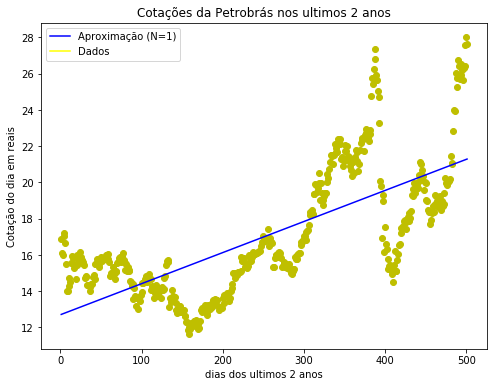
\includegraphics [width=5cm,height=5cm]{Gauss/G1.png}
\includegraphics [width=5cm,height=5cm]{Gauss/G3.png}
\includegraphics [width=5cm,height=5cm]{Gauss/G5.png}
\includegraphics [width=5cm,height=5cm]{Gauss/G10.png}
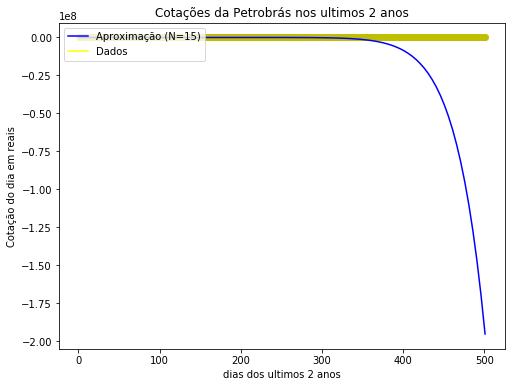
\includegraphics [width=5cm,height=5cm]{Gauss/G15.png}
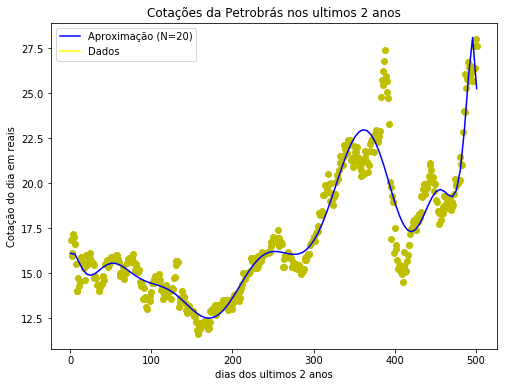
\includegraphics [width=5cm,height=5cm]{Gauss/G20.png}
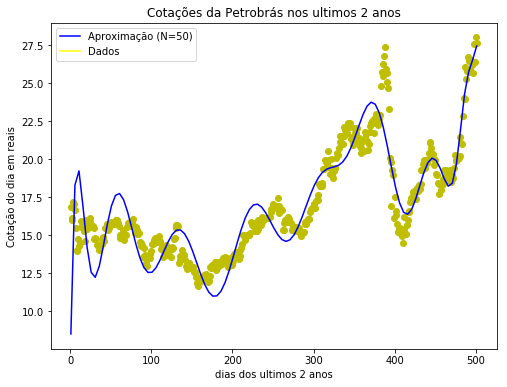
\includegraphics [width=5cm,height=5cm]{Gauss/G50.png}
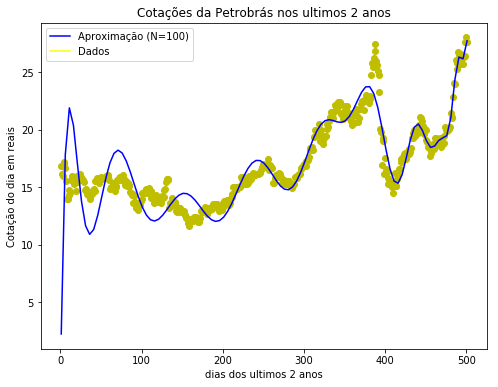
\includegraphics [width=5cm,height=5cm]{Gauss/G100.png}
\end{figure}


\newpage

\item - Analise utilizando-se do método LU.
\begin{figure}[!htb]
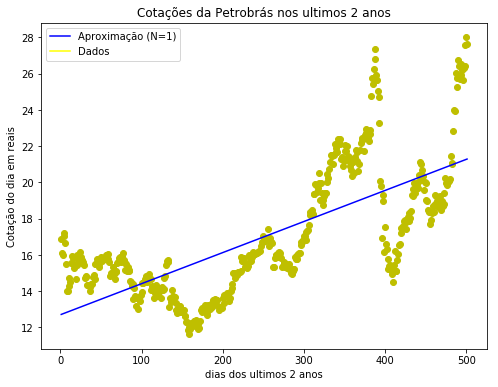
\includegraphics [width=5cm,height=5cm]{LU/G1.png}
\includegraphics [width=5cm,height=5cm]{LU/G3.png}
\includegraphics [width=5cm,height=5cm]{LU/G5.png}
\includegraphics [width=5cm,height=5cm]{LU/G10.png}
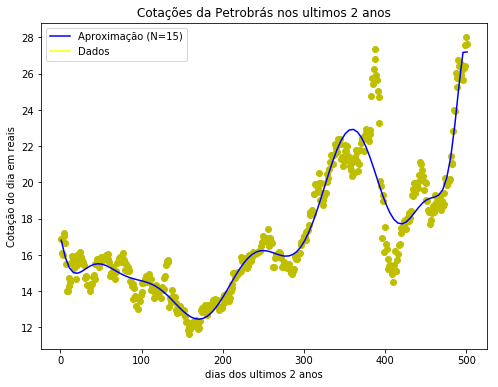
\includegraphics [width=5cm,height=5cm]{LU/G15.png}
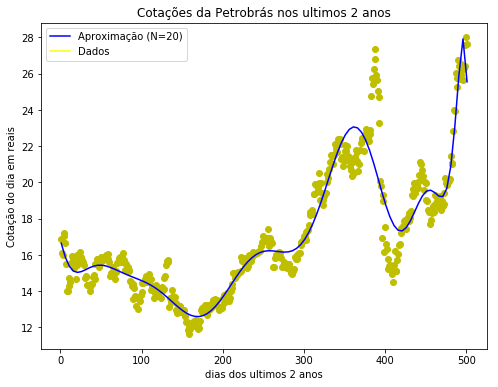
\includegraphics [width=5cm,height=5cm]{LU/G20.png}
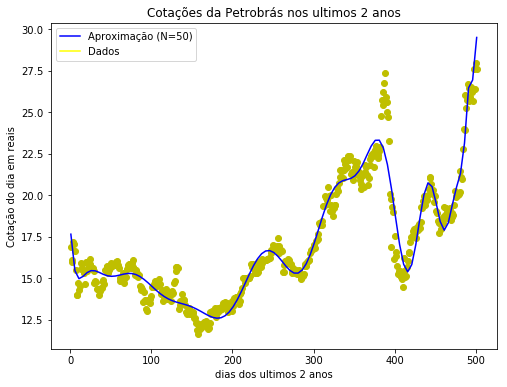
\includegraphics [width=5cm,height=5cm]{LU/G50.png}
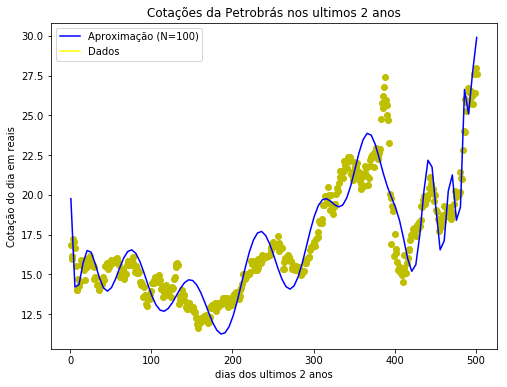
\includegraphics [width=5cm,height=5cm]{LU/G100.png}
\end{figure}

\newpage

\text Definindo as colunas x e y para o método polinomial do item (a), o coeficiente r que pode ser calculado e expresso em porcetagem é:
\begin{table}[h]
\centering
  \begin{tabular}{l|l|lll}
    $Ordem$ $n$ & $Coeficiente$ $r$ & $Coeficiente$ $r$ $em$ $porcetagem$ $(\%)$\\
    \hline
    1 &  0.71092847081604467315 & 71.092\\
    
    3 & 0.7910095119409314065 & 79.100\\
    
    5 & 0.8750227594557078267  & 87.502 \\
    
    10 & 0.9132363941170467756 & 91.323\\
    
    15 &  \sqrt{-110898660834074.66367}    & Não Possui uma raiz real\\
    
    20 & 0.9436191040476386921 & 94.361\\
    
    50 & 0.8960730081149934023 & 89.607\\
    
    100 & 0.8433231181608608121 & 84.332 \\
    \hline
  \end{tabular}
  \caption{coeficiente r em porcetagem para o método de Gauss}
\end{table}

\begin{table}[h]
\centering
  \begin{tabular}{l|l|lll}
    $Ordem$ $n$ & $Coeficiente$ $r$ & $Coeficiente$ $r$ $em$ $porcetagem$ $(\%)$\\
    \hline
    1 &  0.71092847081604467743 & 71.092\\
    
    3 & 0.7910095119409314058 & 79.100\\
    
    5 & 0.87502275945570782376  & 87.502 \\
    
    10 & 0.91323639411704699335 & 91.323\\
    
    15 & 0.94150258009193910986    & 94.150\\
    
    20 & 0.94373292342024341523 & 94.373\\
    
    50 & 0.9656205483094383549 & 96.562\\
    
    100 & 0.88523656133428724256 & 88.523 \\
    \hline
  \end{tabular}
  \caption{coeficiente r em porcetagem para o método LU}
\end{table}

\text Todos os testes acima foram realizados em computador Mac mini (Late 2014).
Com as seguintes configurações;
\item Processador: 1,4 GHz Intel Core i5
\item Memoria: 8 GB 1600 MHz DDR3
\item Sistema Operacional: OSX 10.14.1

\newpage 
Analisando a partir dos resultados obtidos nos itens anteriores, as tentativas de previsão para os próximos 100 dias resultam em:

\item Pelo Método de Gauss:
\begin{figure}[!htb]
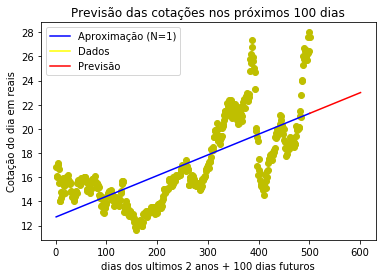
\includegraphics [width=5cm,height=5cm]{PrevisaoG/P1.png}
\includegraphics [width=5cm,height=5cm]{PrevisaoG/P3.png}
\includegraphics [width=5cm,height=5cm]{PrevisaoG/P5.png}
\includegraphics [width=5cm,height=5cm]{PrevisaoG/P10.png}
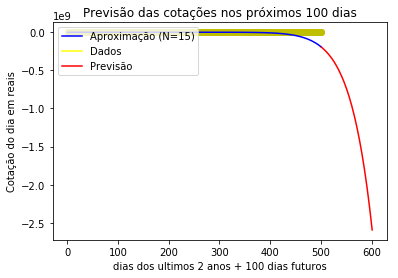
\includegraphics [width=5cm,height=5cm]{PrevisaoG/P15.png}
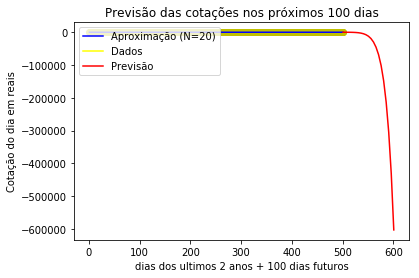
\includegraphics [width=5cm,height=5cm]{PrevisaoG/P20.png}
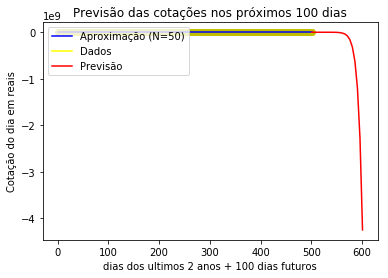
\includegraphics [width=5cm,height=5cm]{PrevisaoG/P50.png}
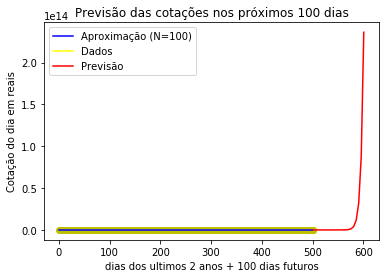
\includegraphics [width=5cm,height=5cm]{PrevisaoG/P100.png}
\end{figure}

\item Pelo Método LU:
\begin{figure}[!htb]
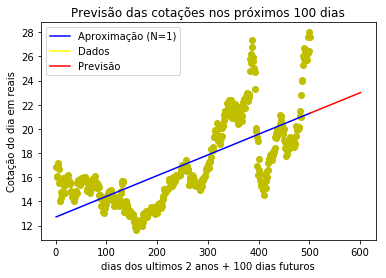
\includegraphics [width=5cm,height=5cm]{PrevisaoLU/P1.png}
\includegraphics [width=5cm,height=5cm]{PrevisaoLU/P3.png}
\includegraphics [width=5cm,height=5cm]{PrevisaoLU/P5.png}
\includegraphics [width=5cm,height=5cm]{PrevisaoLU/P10.png}
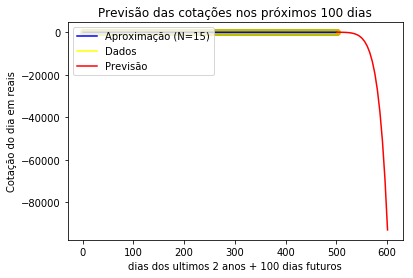
\includegraphics [width=5cm,height=5cm]{PrevisaoLU/P15.png}
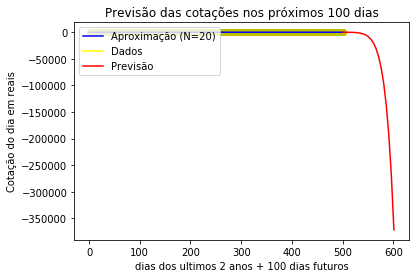
\includegraphics [width=5cm,height=5cm]{PrevisaoLU/P20.png}
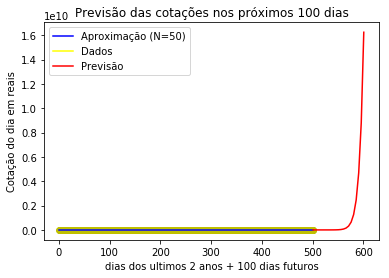
\includegraphics [width=5cm,height=5cm]{PrevisaoLU/P50.png}
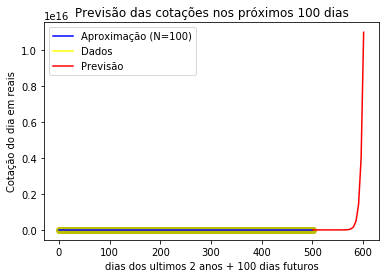
\includegraphics [width=5cm,height=5cm]{PrevisaoLU/P100.png}
\end{figure}

\newpage

\text Como os gráficos demonstram, as tentativas de previsão por ambos os métodos, Gauss e LU, não funcionam bem, conseguindo uma projeção apenas para $N = 1$. Essa falha na previsão se origina de uma falha do Método dos Mínimos Quadrados, que faz que ele não funcione bem para casos em que há ocorrência de erro na "variável dependente" ou em relação entre dados e parâmetros não lineares. 

\end{document}
